\documentclass[11pt] {article}
\usepackage{datetime}
\usepackage{eso-pic}
\usepackage{graphicx}
\usepackage{xcolor}
\usepackage{atbegshi,picture}
\usepackage{geometry}
\usepackage{ragged2e}
\graphicspath{ { ./sdcard/Documents/fwc/} }
\geometry{a4paper,total={200mm,225mm},left=25mm,right=30mm}

\begin {document}

\AtBeginShipout{\AtBeginShipoutUpperLeft{%
	\put(\dimexpr\paperwidth-1cm\relax,-1.5cm){\makebox[0pt][r]{EXEMPLAR PROBLEMS}}%
}}

\begin{center}
\color{cyan}
	{\Large EXERCISE 7.4}
\end{center}

\begin {enumerate}
\item Find all the angles of an equilateral triangle.

\begin{minipage}[h]{0.65\linewidth}
\item The image of an object placed at a point A before a plane mirror LM is seen at the point B by an observer at D as shown in Fig. 7.12. Prove that the image is as far behind the mirror as the object is in front  of the mirror.                              
\end{minipage}
\hfill
\begin{minipage}[h]{0.35\linewidth}
	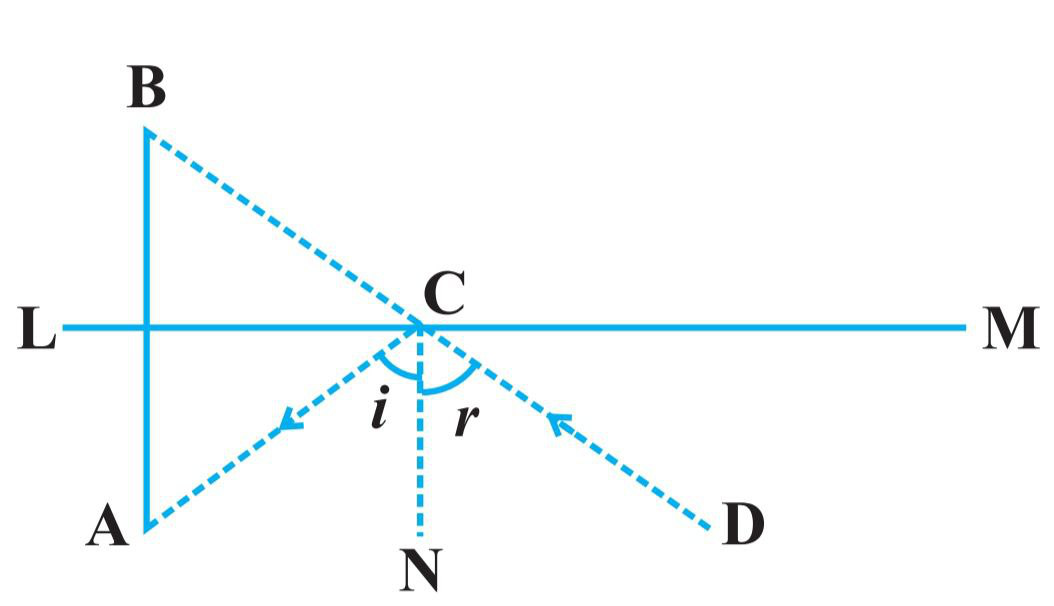
\includegraphics[scale=0.14]{7A}
\end{minipage}

[\textcolor{cyan}{Hint:} CN is normal to the mirror. Also, angle of incidence = angle of reflection].

\item ABC is an isosceles triangle with AB = AC and D is a point on BC such that AD $\perp$  BC (Fig. 7.13). To prove that $\angle$ BAD = $\angle$ CAD, a student proceeded as follows:

\begin{minipage}[h]{0.70\linewidth}
In $\triangle$  ABD and $\triangle$  ACD,

\hspace{2.6 cm}  AB = AC \hspace{1cm}(Given)

\hspace{2.5cm} $\angle$ B = $\angle$C \hspace{1cm}(because AB = AC)

and \hspace{1.3cm}  $\angle$ ADB = $\angle$ ADC

Therefore, \hspace{0.3 cm}$\triangle$  ABD $\cong$  $\triangle$ ACD (AAS)

So, \hspace{1.4cm}  $\angle$ BAD = $\angle$ CAD (CPCT)

What is the defect in the above arguments?

[\textcolor{cyan}{Hint:} Recall how $\angle$ B = $\angle$ C is proved whenAB = AC]
\end{minipage}
\hfill
\begin{minipage}[h]{0.30\linewidth}                             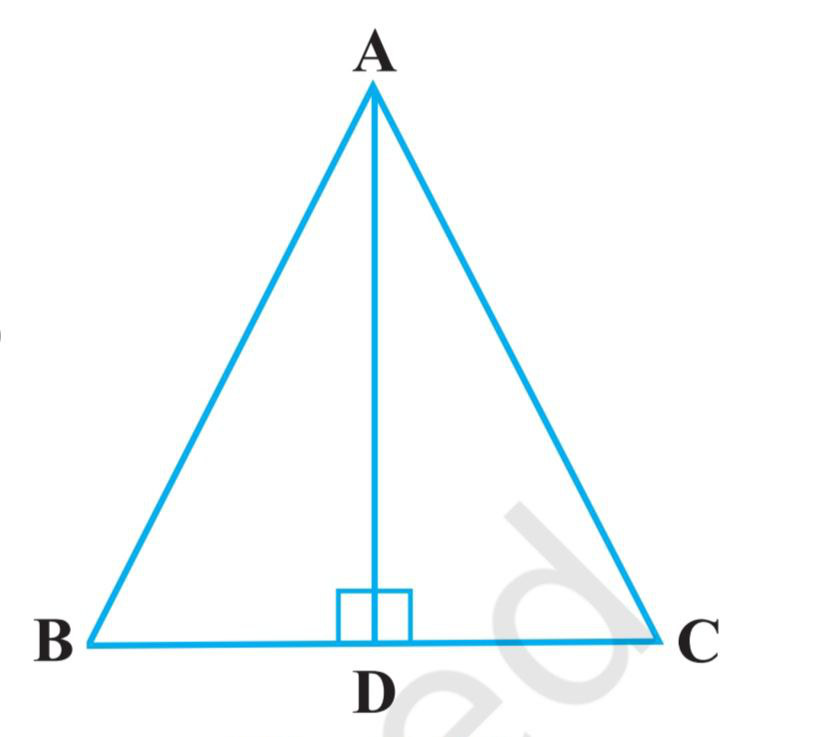
\includegraphics[scale=0.14]{7B}          
\end{minipage}
\item P is a point on the bisector of $\angle$ ABC. If the line through P, parallel to BA meet BC at Q, prove that BPQ is an isosceles triangle.
\item ABCD is a quadrilateral in which AB = BC and AD = CD. Show that BD bisects both the angles ABC and ADC.
\item ABC is a right triangle with AB = AC. Bisector of $\angle$ A meets BC at D. Prove that BC = 2 AD
\item O is a point in the interior of a square ABCD suchthat OAB is an 

equilateral triangle. Show that $\triangle$  OCD is an isosceles triangle.
\item ABC and DBC are two triangles on the same base BC such that A and D lie on the opposite sides of BC, AB = AC and DB = DC. Show that AD is the perpendicular bisector of BC.
\item ABC is an isosceles triangle in which AC = BC. AD and BE are respectively two altitudes to sides BC and AC. Prove that AE = BD.
\item Prove that sum of any two sides of a triangle is greater than twice the median with respect to the third side.
\item Show that in a quadrilateral ABCD, AB + BC + CD + DA $<$ 2 (BD + AC)
\item Show that in a quadrilateral ABCD,

AB + BC + CD + DA $>$ AC + BD
\item In a triangle ABC, D is the mid-point of side AC such that BD = $\frac{1}{2}$AC. Show that

$\angle$ ABC is a right angle.
\item In a right triangle, prove that the line-segment joining the mid-point of the hypotenuse to the opposite vertex is half the hypotenuse.
\item Two lines l and m intersect at the point O and P is a point on a line n passing through the point O such that P is equidistant from l and m. Prove that n is the bisector of the angle formed by l and m.
\item Line segment joining the mid-points M and N of parallel sides AB and DC, respectively of a trapezium ABCD is perpendicular to both the sides AB and DC. Prove that AD = BC.
\item ABCD is a quadrilateral such that diagonal AC bisects the angles A and C. Prove that AB = AD and CB = CD.
\item ABC is a right triangle such that AB = AC and bisector of angle C intersects the side AB at D. Prove that AC + AD = BC.
\item AB and CD are the smallest and largest sides of a quadrilateral ABCD. Out of $\angle$ B and $\angle$ D decide which is greater.
\item Prove that in a triangle, other than an equilateral triangle, angle opposite the longest side is greater than $\frac{2}{3}$ of a right angle.
\item ABCD is quadrilateral such that AB = AD and CB = CD. Prove that AC is the perpendicular bisector of BD.



\end{enumerate}
\end{document}
